\documentclass[fleqn]{article}
\usepackage[x11names, rgb]{xcolor}
\usepackage[utf8]{inputenc}
\usepackage{tikz}
\usepackage{amsmath}
\usepackage{geometry}
\usepackage{fancyhdr}
\usepackage{amsmath,amsthm,amssymb}
\usepackage{graphicx}
\usepackage{hyperref}
\usepackage{lipsum}
\usepackage{ulem}
\usepackage{comment}
\usepackage{enumerate}
\usepackage{titlesec}
\usepackage{boolexpr,pdftexcmds,trace}
\usepackage{pgfplotstable}
\usepackage{standalone}
\makeatletter

\graphicspath{{./screenshots/}}
\DeclareGraphicsExtensions{.png}   

\usetikzlibrary{snakes,arrows,shapes}
\newwrite\dotfile

\begingroup
  \catcode`\[ = 1\relax
  \catcode`\] = 2\relax
  \catcode`\{ = 12\relax
  \catcode`\} = 12 \relax
  \gdef\OpenBrace[{]
  \gdef\CloseBrace[}]
\endgroup

% custom commands
\newcommand{\leadingzero}[1]{\ifnum #1<10 0#1\else#1\fi}
\newcommand{\gerdate}[3]{\leadingzero{#1}.\leadingzero{#2}.\leadingzero{#3}}
\newcommand{\gertoday}{\gerdate{\the\day}{\the\month}{\the\year}}
\newcommand*{\bfrac}[2]{\genfrac{}{}{0pt}{}{#1}{#2}}
\newcommand{\R}{\mathbb{R}}
\newcommand{\N}{\mathbb{N}}
\newcommand{\Q}{\mathbb{Q}}
\newcommand{\Z}{\mathbb{Z}}
\newcommand{\dotarrow}[0]{}

\newenvironment{graphviz}[1]%
{%
\switch
\case{\pdf@strcmp{#1}{graph}}
    \renewcommand{\dotarrow}[0]{--}
\case{\pdf@strcmp{#1}{strict graph}}
    \renewcommand{\dotarrow}[0]{--}
\case{\pdf@strcmp{#1}{digraph}}
    \renewcommand{\dotarrow}[0]{->}
\case{\pdf@strcmp{#1}{strict digraph}}
    \renewcommand{\dotarrow}[0]{->}
\endswitch

\immediate\openout\dotfile=tmp.dot%
\newcommand{\node}[2]{%
\immediate\write\dotfile{##1 \dotarrow \OpenBrace##2\CloseBrace}%
}%
%
\immediate\write\dotfile{#1 \OpenBrace}
}%
{\immediate\write\dotfile{\CloseBrace}%
\immediate\closeout\dotfile%
\immediate\write18{dot2tex --figonly tmp.dot > tmp.tex}%
\input{tmp.tex}%
}

\setcounter{section}{0}
\setcounter{subsection}{0}
\pagestyle{fancy}

\lhead{Tobias Knöppler, Klaus Ziegert}
\chead{}
\rhead{\gertoday}
\lfoot{}
\cfoot{\thepage}
\rfoot{}
%\setlength{\mathindent}{0pt}

% document specific settings
%\renewcommand{\thesection}{}
\renewcommand{\thesubsection}{\arabic{section}. \alph{subsection})}
\renewcommand{\thesubsubsection}{\roman{subsubsection})}
\titleformat{\subsubsection}[runin]{\normalfont\normalsize\bfseries}{\thesubsubsection}{1em}{}

\title{Visualisierung}
\begin{document}
\section{Anwendungsbeispiel}
\begin{center}
mpirun -np 8 circle 20\\
\begin{tabular}{|l|l|}            \hline\hline
Before & After\\
rank 0: 22 & rank 0: 1\\ 
rank 0: 12 & rank 0: 5\\
rank 0: 11 & rank 0: 7\\
rank 1: 1 & rank 1: 13\\
rank 1: 5 & rank 1: 6\\
rank 1: 7 & rank 1: 23\\
rank 2: 13 & rank 2: 14\\
rank 2: 6 & rank 2: 6\\
rank 2: 23 & rank 2: 3\\
rank 3: 14 & rank 3: 1\\
rank 3: 6 & rank 3: 14\\
rank 3: 3 & rank 4: 20\\
rank 4: 1 & rank 4: 5\\
rank 4: 14 & rank 5: 1\\
rank 5: 20 & rank 5: 11\\
rank 5: 5 & rank 6: 11\\
rank 6: 1 & rank 6: 5\\
rank 6: 11 & rank 7: 22\\
rank 7: 11 & rank 7: 12\\
rank 7: 5 & rank 7: 11\\
\hline
\end{tabular}
\end{center}
\section{Visualisierung}
Die folgende Farbkodierung gilt für alle Screenshots:\\
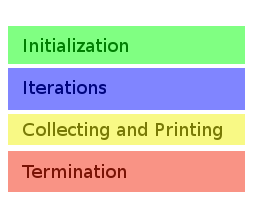
\includegraphics[scale=0.4]{caption}

\subsection{}%subsection name}\label{label}
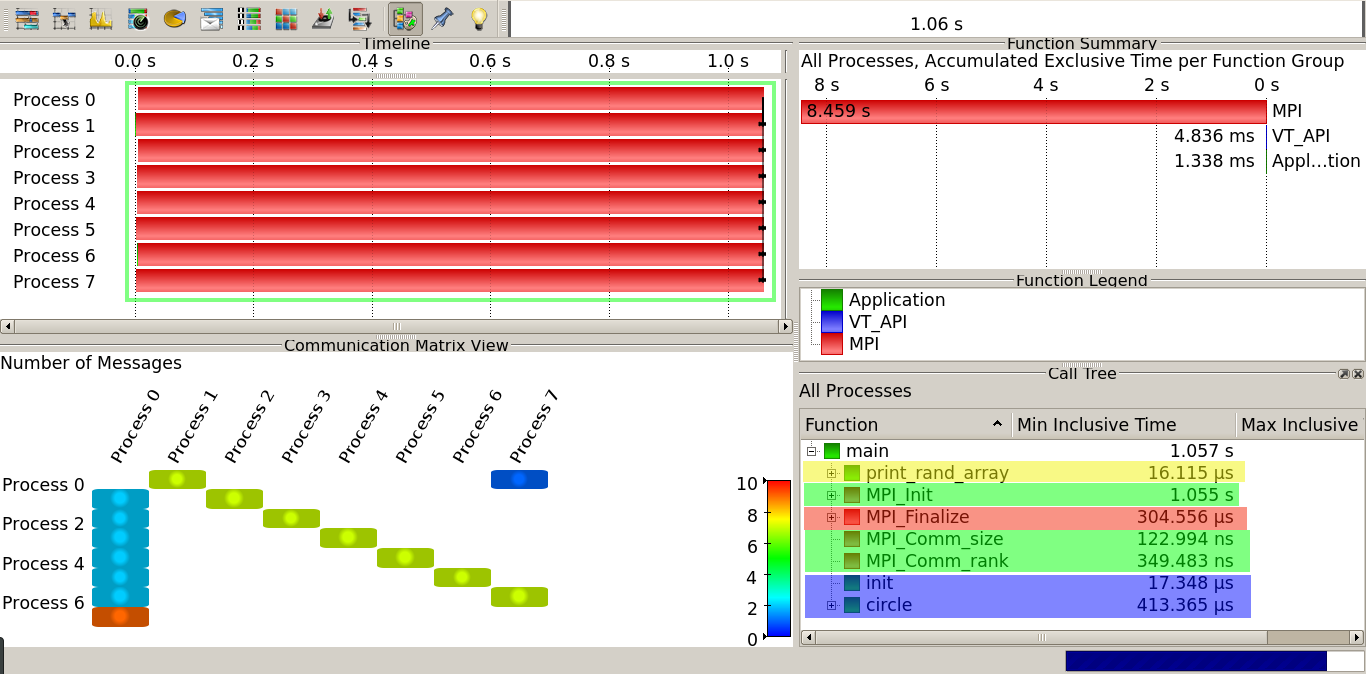
\includegraphics[width=\textwidth]{vampir1}
Links oben, in dem grünen Kasten ist dargestellt, zu welcher Zeit sich jeder Prozess innerhalb von MPI-Funktionen, VT\_API-Funktionen oder programmeigenen Funktionen aufhielt. Deutlich erkennbar ist dabei, dass der Parallelisierungsoverhead (v.a. Initialisierung) in diesem Fall wesentlich mehr Zeit in Anspruch nahm, als der eigentliche Programmcode (Das berechnen, Vergleichen und Ausgeben der Zufallsvariablen).\\
Rechts oben ist dasselbe noch einmal für das Programm insgesamt aufgeführt.\\
Links unten ist in einer Matrix dargestellt, wie oft jedes Paar von Prozessen miteinander kommuniziert hat. Erkennbar ist, dass jeder Prozess mit dem letzten kommuniziert hat, da dieser den anderen einmal pro Iteration die Abbruchvariable mitgeteilt hat. Ansonsten hat jeder Prozess nur je einmal mit seinem Vorgänger und Nachfolger kommuniziert.\\
Rechts unten ist die Zeit aufgeführt, die das Programm in jeder Funktion verbracht hat. Ich habe farbig markiert, welche Funktion zu welcher Programmphase gehört.

\subsection{}%subsection name}\label{label}
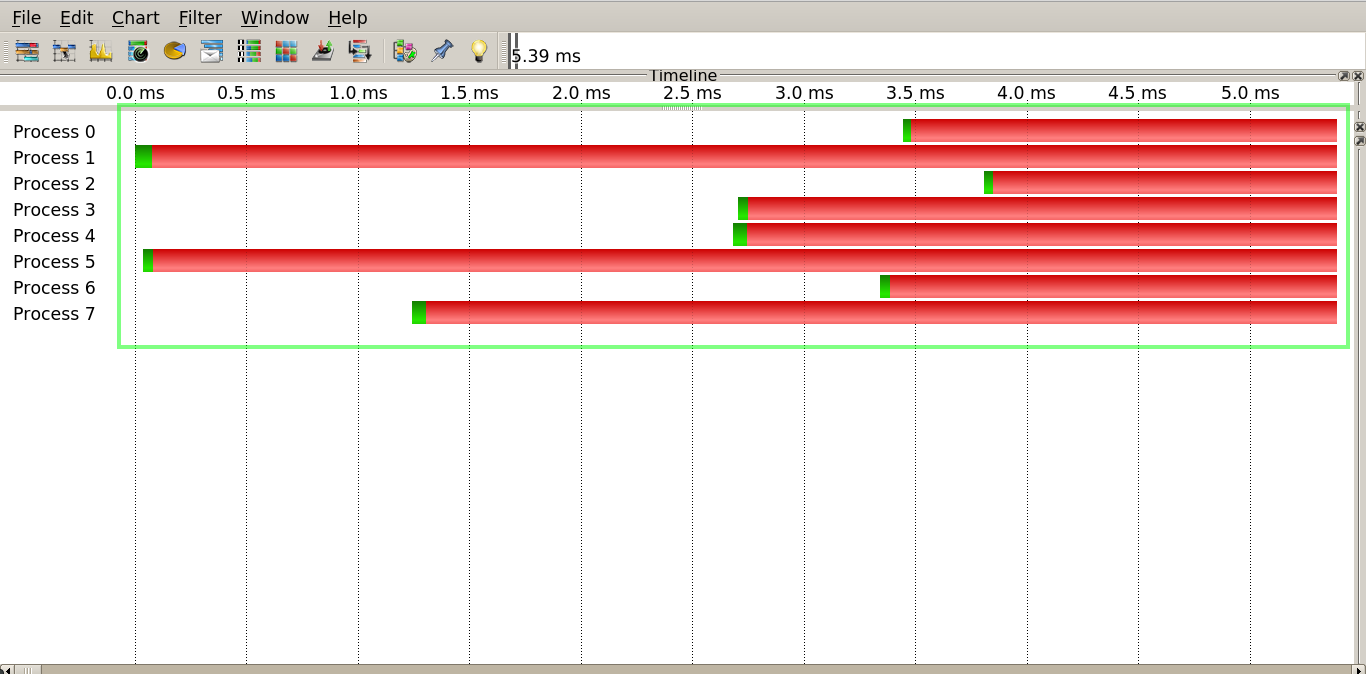
\includegraphics[width=\textwidth]{vampir2}
Hier ist zu sehen, wann die einzelnen Prozesse initialisiert wurden. Dies findet offensichtlich in der Initialisierungsphase statt.

\subsection{}%subsection name}\label{label}
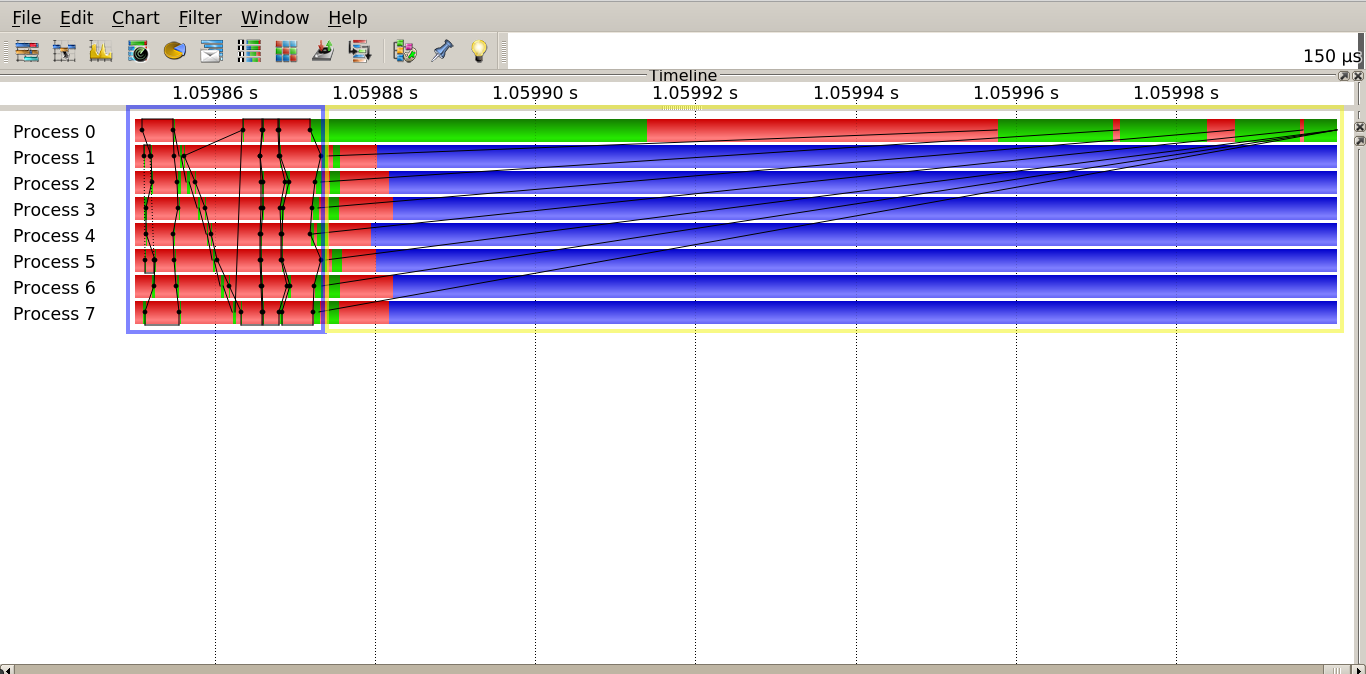
\includegraphics[width=\textwidth]{vampir3}
Hier ist dargestellt, zu welcher Zeit die Prozesse arbeiteten (grün), von MPI blockiert waren (rot) oder schon terminiert hatten (blau). Im Bereich innerhalb des blauen Kastens befindet sich das Programm in der while-Schleife während welcher die Zufallsvariablen ausgetauscht werden.\\
Im Bereich innerhalb des gelben Kastens (evtl. schwer zu sehen) befindet sich das Programm in der Ausgabephase (alle Prozesse außer dem Masterprozess haben bereits terminiert).
\subsection{}%subsection name}\label{label}
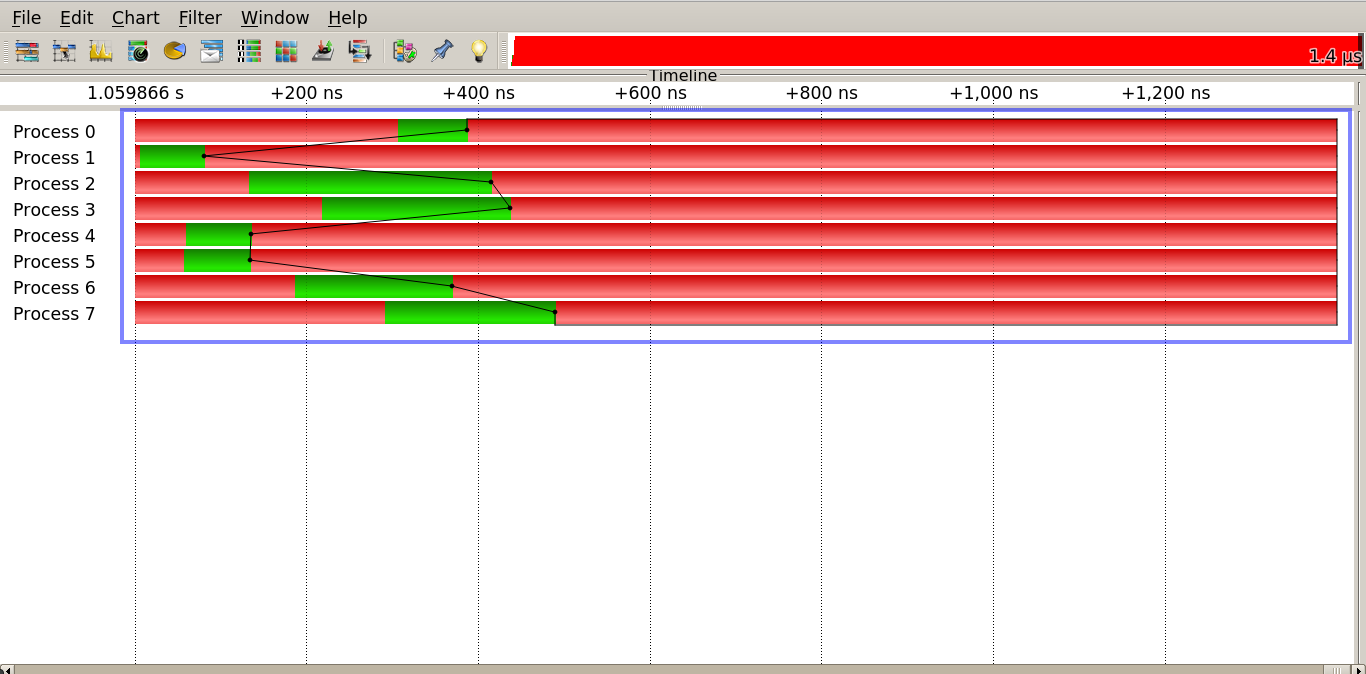
\includegraphics[width=\textwidth]{vampir4}
Hier ist eine Iteration der while-Schleife zu sehen. Die durch die schwarze Linie verbundenen Punkte markieren die Zeitpunkte an denen jeder Prozess die Barrier erreicht hat.




\end{document}
